\section{XGBoost}\label{sec:xgb}

\subsection{Giới thiệu về XGBoost}
Khác với bagging, \textit{boosting} xây dựng các cây \textbf{tuần tự}: mỗi cây $f_m$ học phần sai số (gradient âm của hàm mất mát) mà các cây trước chưa giải thích được, rồi được cộng vào mô hình với tốc độ học $\eta$. XGBoost \cite{chen2016} cực tiểu hóa hàm mục tiêu có số hạng phạt độ phức tạp của cây ($T_f$: số lá, $w_j$: giá trị tại lá):
\begin{equation}
    F_m(\mathbf{x}) = F_{m-1}(\mathbf{x}) + \eta \, f_m(\mathbf{x}), \qquad
    \mathcal{L} = \sum_{i=1}^{n} \ell\big(y_i, \hat{y}_i\big) + \sum_{m} \Big(\gamma T_{f_m} + \tfrac{1}{2}\lambda \sum_{j} w_j^2\Big)
\end{equation}
Nhờ khai triển Taylor bậc hai (gradient $g_i$, hessian $h_i$), giá trị tối ưu tại lá có công thức đóng $w_j^{*} = -\sum_{i \in I_j} g_i / (\sum_{i \in I_j} h_i + \lambda)$, và mức \textit{gain} khi tách nút được tính trực tiếp từ tổng $g_i$, $h_i$ ở hai nhánh. XGBoost còn hỗ trợ lấy mẫu con theo dòng/cột (\texttt{subsample}, \texttt{colsample\_bytree}), ràng buộc \texttt{min\_child\_weight}, thuật toán histogram và \texttt{scale\_pos\_weight} cho dữ liệu mất cân bằng.

\begin{figure}[H]
\centering
\begin{tikzpicture}[
    node distance=0.4cm and 0.8cm,
    box/.style={rectangle, rounded corners, draw=black!60, minimum height=0.7cm, minimum width=1.6cm, align=center, font=\small},
    arrow/.style={-{Stealth[length=2mm]}, thick}
]
\node[box, fill=orange!15] (f0) {$F_0$};
\node[box, fill=blue!10, right=of f0] (t1) {Cây $f_1$};
\node[box, fill=blue!10, right=of t1] (t2) {Cây $f_2$};
\node[right=of t2] (dots) {$\cdots$};
\node[box, fill=blue!10, right=of dots] (tM) {Cây $f_M$};
\node[box, fill=green!12, right=of tM] (out) {$\hat{p} = \sigma\big(F_0 + \eta \sum_m f_m\big)$};
\draw[arrow] (f0) -- (t1); \draw[arrow] (t1) -- (t2); \draw[arrow] (t2) -- (dots); \draw[arrow] (dots) -- (tM); \draw[arrow] (tM) -- (out);
\end{tikzpicture}
\caption{Cơ chế boosting: các cây được xây dựng tuần tự, mỗi cây học phần sai số còn lại}
\end{figure}

\begin{table}[H]
\centering
\begin{adjustbox}{max width=\textwidth}
\begin{tabular}{|p{7cm}|p{7cm}|}
\hline
\textbf{Ưu điểm} & \textbf{Nhược điểm} \\
\hline
Thường chính xác nhất trên dữ liệu bảng & Nhiều siêu tham số, cần tuning cẩn thận \\
\hline
Chính quy hóa sẵn trong hàm mục tiêu & Dễ overfit nếu cây sâu, tốc độ học lớn \\
\hline
Nhanh (histogram), hỗ trợ \texttt{scale\_pos\_weight} & Khó diễn giải hơn mô hình tuyến tính, cây đơn \\
\hline
\end{tabular}
\end{adjustbox}
\caption{Ưu và nhược điểm của XGBoost}
\end{table}

\subsection{Mã nguồn và huấn luyện}
\begin{lstlisting}[style=pythonstyle, caption={Khởi tạo XGBoost trong \texttt{src/models.py}}]
if model_name == "xgboost":
    # XGBoost khong co class_weight, dung scale_pos_weight thay the.
    return XGBClassifier(
        objective="binary:logistic",
        eval_metric="logloss",
        n_estimators=100, learning_rate=0.1, max_depth=6,
        tree_method="hist",
        scale_pos_weight=balance_ratio or 1.0,   # ~2,77 khi dung class weight
        random_state=random_state, n_jobs=1,
    )
\end{lstlisting}

\texttt{RandomizedSearchCV} (không gian tìm kiếm ở Mục~\ref{sec:exp4}) thử 60 tổ hợp trên 5 fold, chọn theo PR-AUC. Cấu hình tốt nhất: 271 cây, \texttt{max\_depth=3}, \texttt{learning\_rate=0,023}, \texttt{min\_child\_weight=5}, \texttt{subsample=0,82}, \texttt{colsample\_bytree=0,96}, \texttt{reg\_lambda=0,79}. So với mặc định (100 cây sâu 6, tốc độ học 0,1), mô hình được chọn dùng nhiều cây nông hơn với tốc độ học nhỏ hơn -- một cấu hình ít overfit hơn.

\subsection{Kết quả và đánh giá}

\subsubsection{Kết quả cross-validation qua các giai đoạn}
\begin{table}[H]
\centering
\small
\begin{adjustbox}{max width=\textwidth}
\begin{tabular}{|l|c|c|c|c|c|c|}
\hline
\textbf{Cấu hình} & \textbf{Precision} & \textbf{Recall} & \textbf{F1} & \textbf{ROC-AUC} & \textbf{PR-AUC} & \textbf{F1 train} \\
\hline
Baseline & 0,650 & 0,520 & 0,578 & 0,841 & 0,653 & 0,760 \\
\hline
+ Class weight & 0,545 & 0,747 & 0,630 & 0,839 & 0,653 & 0,792 \\
\hline
+ Tuning & 0,520 & 0,806 & 0,632 & 0,850 & 0,671 & 0,657 \\
\hline
+ Ngưỡng 0,57 (out-of-fold) & 0,562 & 0,741 & \textbf{0,639} & 0,850 & 0,671 & -- \\
\hline
\end{tabular}
\end{adjustbox}
\caption{XGBoost: kết quả validation (trung bình 5 fold) qua từng bước}
\end{table}

Class weight mang lại phần lớn mức tăng F1 (+0,053, Recall từ 0,520 lên 0,747). Tuning không tăng thêm nhiều F1 (+0,002) nhưng tăng PR-AUC và ROC-AUC ở cả 5 fold (+0,018 và +0,011), đồng thời thu hẹp khoảng cách F1 train--validation từ 0,16 xuống 0,03. Sau tuning, XGBoost có PR-AUC và ROC-AUC cross-validation cao nhất trong bốn mô hình, nên được chọn làm mô hình chính trước khi dùng tập test.

\subsubsection{Kết quả trên tập test}
\begin{table}[H]
\centering
\begin{minipage}[t]{0.56\textwidth}
\centering
\small
\begin{adjustbox}{max width=\textwidth}
\begin{tabular}{|l|c|c|c|c|}
\hline
\textbf{Lớp} & \textbf{Precision} & \textbf{Recall} & \textbf{F1-score} & \textbf{Support} \\
\hline
Không rời bỏ (0) & 0,90 & 0,78 & 0,83 & 1.035 \\
\hline
Rời bỏ (1) & 0,55 & 0,75 & 0,63 & 374 \\
\hline
Accuracy & & & 0,77 & 1.409 \\
\hline
Macro avg & 0,72 & 0,76 & 0,73 & 1.409 \\
\hline
Weighted avg & 0,80 & 0,77 & 0,78 & 1.409 \\
\hline
\end{tabular}
\end{adjustbox}
\caption{XGBoost: kết quả phân loại trên tập test (ngưỡng 0,57; ROC-AUC 0,846; PR-AUC 0,662)}
\end{minipage}\hfill
\begin{minipage}[t]{0.42\textwidth}
\centering
\small
\begin{adjustbox}{max width=\textwidth}
\begin{tabular}{|c|c|c|c|}
\cline{3-4}
\multicolumn{2}{c|}{} & \multicolumn{2}{c|}{\textbf{Dự đoán}} \\
\cline{3-4}
\multicolumn{2}{c|}{} & Không rời bỏ & Rời bỏ \\
\hline
\multirow{2}{*}{\textbf{Thực tế}} & Không rời bỏ & \cellcolor{blue!30}806 & 229 \\
\cline{2-4}
 & Rời bỏ & 94 & \cellcolor{blue!30}280 \\
\hline
\end{tabular}
\end{adjustbox}
\caption{XGBoost: Confusion Matrix trên tập test}
\end{minipage}
\end{table}

XGBoost phát hiện được nhiều khách hàng rời bỏ nhất (280/374, Recall 0,749) và có F1 lớp rời bỏ cao nhất (0,634). Đổi lại có 229/1.035 khách hàng ở lại bị cảnh báo nhầm. Nếu dùng ngưỡng ưu tiên Recall (F2, ngưỡng 0,37), mô hình phát hiện 329/374 khách hàng rời bỏ (Recall 0,880) với Precision 0,460.

\subsubsection{Feature Importance}
\begin{figure}[H]
\centering
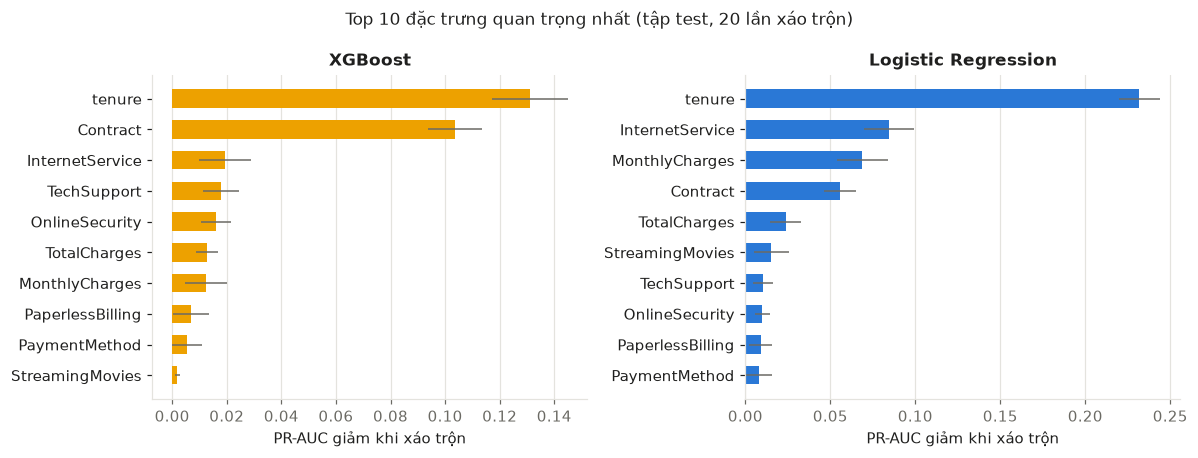
\includegraphics[width=\textwidth]{img/nb_permutation_importance.png}
\caption{Permutation importance trên tập test của XGBoost và Logistic Regression: mức giảm PR-AUC khi xáo trộn từng đặc trưng (vạch: độ lệch chuẩn qua 20 lần xáo trộn)}
\label{fig:perm}
\end{figure}

Hai cách đo cho kết quả khác nhau đáng kể:
\begin{itemize}
    \item \textbf{Permutation importance} (Hình~\ref{fig:perm}) xếp \texttt{tenure} quan trọng nhất (PR-AUC giảm 0,131 khi xáo trộn), tiếp theo là \texttt{Contract} (0,104), rồi \texttt{InternetService}, \texttt{TechSupport}, \texttt{OnlineSecurity} (0,016--0,019).
    \item \textbf{Gain importance} (thuộc tính \texttt{feature\_importances\_} của XGBoost) xếp \texttt{Contract} chiếm 50\% tổng gain, còn \texttt{tenure} chỉ 2\%.
\end{itemize}
Khác biệt này đến từ cách tính: gain chỉ cộng mức cải thiện tại các lần tách nút, nên đặc trưng một lần tách lớn như \texttt{Contract\_Month-to-month} được đánh giá rất cao; \texttt{tenure} là đặc trưng liên tục được dùng ở nhiều lần tách nhỏ (cây sâu 3, 271 cây), mỗi lần đóng góp ít gain nhưng tổng ảnh hưởng lên dự đoán lại lớn nhất. Permutation importance đo trực tiếp ảnh hưởng lên chất lượng dự đoán trên tập test nên đáng tin cậy hơn để kết luận mức độ quan trọng.

\subsubsection{Nhận xét và đánh giá}
\textbf{Điểm mạnh}
\begin{itemize}
    \item Mô hình tốt nhất trên tập test ở F1 (0,634), Recall (0,749), ROC-AUC (0,846) và PR-AUC (0,662), khớp với lựa chọn dựa trên cross-validation.
    \item Kết quả test rất sát cross-validation (PR-AUC 0,671 so với 0,662; ROC-AUC 0,850 so với 0,846): quy trình chọn mô hình không bị overfit vào các fold.
    \item Sau tuning gần như không overfit (khoảng cách F1 train--validation 0,03), mô hình gọn (khoảng 0,3 MB).
\end{itemize}

\textbf{Hạn chế}
\begin{itemize}
    \item Chênh lệch với Random Forest và Decision Tree trên tập test nhỏ (F1 0,005--0,010), có thể chỉ là nhiễu với 374 khách hàng rời bỏ.
    \item Ở cấu hình mặc định, XGBoost overfit (F1 train 0,760 so với validation 0,578) và Feature Engineering làm giảm hiệu năng: mô hình cần tuning cẩn thận.
    \item Khó diễn giải từng dự đoán hơn Logistic Regression và Decision Tree; các cách đo importance khác nhau cho thứ hạng khác nhau.
\end{itemize}

\textbf{Hướng cải thiện}
\begin{enumerate}
    \item Dùng SHAP \cite{lundberg2017} để giải thích từng khách hàng và nhất quán hóa mức độ quan trọng của đặc trưng.
    \item Thử LightGBM, CatBoost (xử lý trực tiếp biến phân loại) hoặc dừng sớm (\textit{early stopping}) thay cho cố định số cây.
    \item Hiệu chỉnh xác suất (\textit{calibration}) để xác suất rời bỏ có thể dùng trực tiếp trong tính toán chi phí -- lợi ích của chiến dịch giữ chân.
\end{enumerate}
